\documentclass[11pt]{article}
%\begin{document}
\usepackage{amsmath,amsthm,amssymb,graphicx}
\usepackage{hyperref}
\usepackage[numbers]{natbib}
\usepackage{float}
\usepackage{bbm}

\topmargin -.7in
\textwidth 6.5in
\textheight 9.5in
\evensidemargin 0in
\oddsidemargin 0in

\pagenumbering{arabic}

\begin{document}
 %\dspace 12pt
% \sspace 6pt
%\sdspace 11pt

\pagestyle{empty}
%\flushbottom
%\begin{document}

%\centerline{\Huge\bf !!! NOTE ROOM CHANGE !!!}

\vspace{-.5in}

\large
\begin{center}
{\bf Yale University \\ Computer Vision\vspace{.2in} \\
Term Project}\large\vspace{.3in} \\
{\bf Leon Lixing Yu}\vspace{.3in}\\ 

%Department of Electrial Engineering\\
%Yale University\vspace{.2in}\\
 % title
% {\Large \bf A safe Database by hardware information flow tracking}
{\Large \bf What is so good about Principle Component Analysis?}
\vspace{.3in}\\ 

\end{center}

\vspace{.25in}

\section{Introduction}


\par
The goal of this project is to show the advantages or disadvantages of using Principle Component Analysis (PCA) to reduce the dimensionality of the chosen datasets in classification problems. The catalyst behind this project idea is that in assignment 3, we practiced how to use Singular Value Decomposition (SVD) to reduce observations with 3 features to 2 features. We also learnt that PCA does not work well while observations is distributed over a manifold. However, after extracting the principle components, the assignment does not guide us through how to apply the principle components to either classification or regression problems, and how it can impact the prediction accuracy. Out of my own couriosity, I decide to use Support Vector Machine (SVM) as my classification method and apply principle components to train the model. Once the training is done, I apply the chosen testing set to verify the accuracy and compare it against SVM-only results. The results include the training and testing time, testing accuracy, and total program runtime. In the following paragraphs, I will refer to the PCA-enabled SVM as PCA-SVM and direct SVM application as SVM-Only. This report first walks through how the datasets are chosen and then discuss the implementation details. Section 4 presents the benchmark results and discusses the pros and cons of applying PCA for the specific datasets. 
Lastly, I draw conclusion on the pros and cons of doing dimensionality reduction for classification problems. 

\section{Datasets}
 Throughout assignment 3, we have been addressing the fact that not every dataset is compatiable with PCA. The dimensionality reduction only works well when the observations follows a multivariate gaussian distribution. Since we have explored disvantages of PCA in terms of observations' distribution, I try to avoid choosing datasets that form a manifold distribution.\par 
The datasets I have chosen are Iris flower dataset, overian cancer datset, and proteomics dataset. Iris flower dataset is a multivariate gaussian dataset (see figure 1 below) composed by Ronald Fischer in 1936.The dataset is used to quantify the three species of iris flower. 

\begin{figure}[H]
\centering
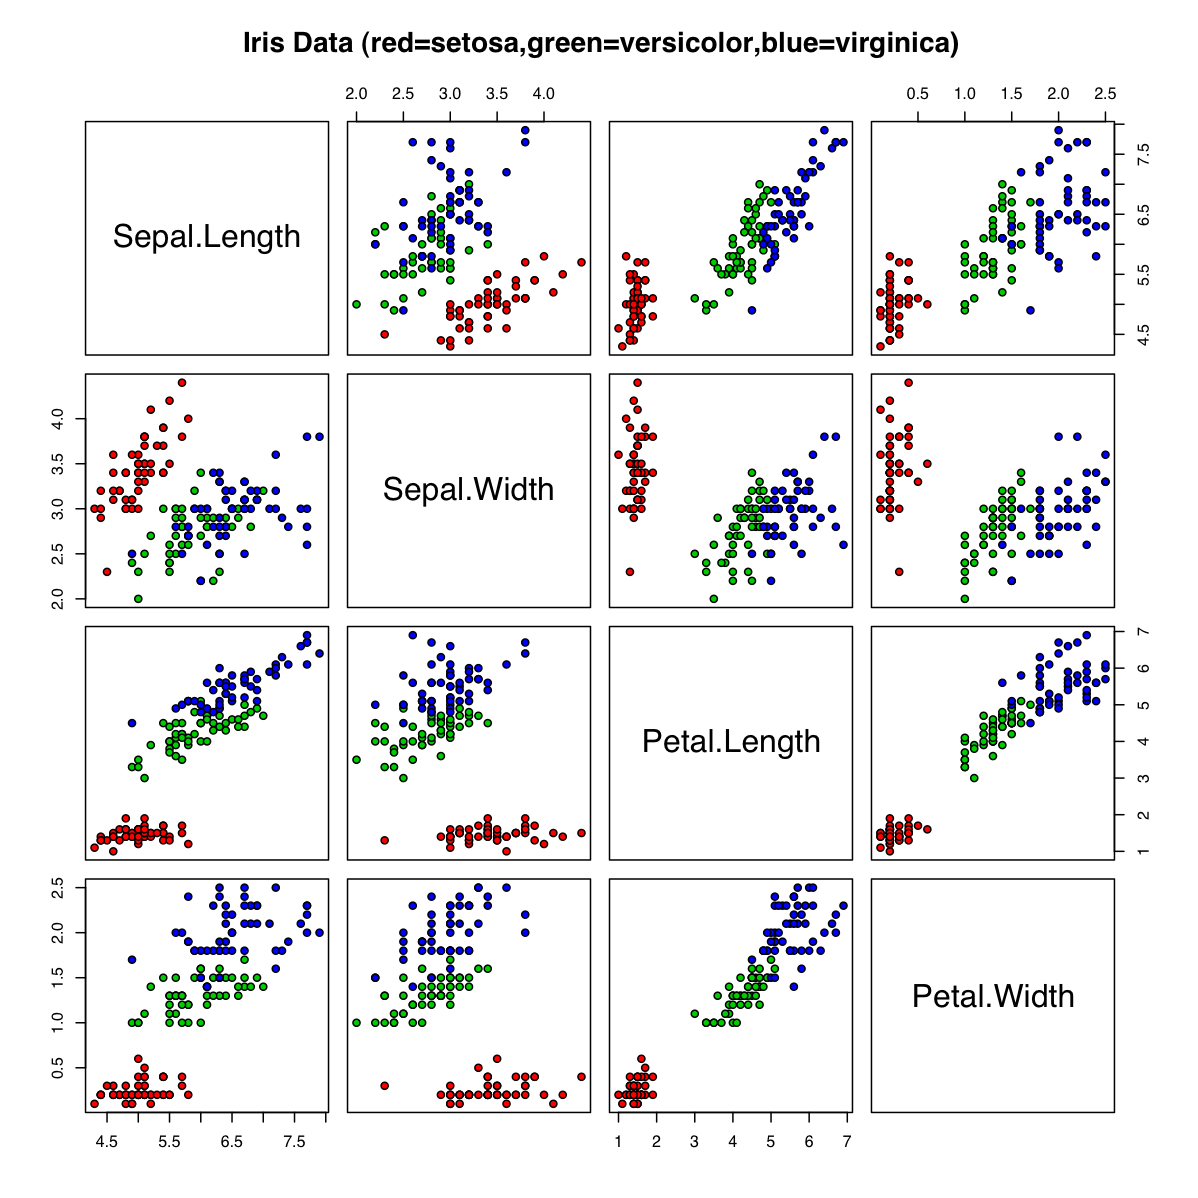
\includegraphics[width=120mm]{iris.jpg}
\caption{ Fischer's iris flower dataset scatter plot. Each panel displays 2 features for 3 different species.The graph is referened from $http://en.wikipedia.org/wiki/Iris\_flower\_data\_set$ \label{problem1Pic2}}
\end{figure}

The set has 150 observations, each with four features. The labels are the flower names, setosa, versicolor, and virginica. Though it is a legacy dataset, its compact size is highly useful to validate the correctness of my code as well as to show the dimensionality reduction effects on tiny datasets. One of the major drawback of choosing this dataset is that it only has 150 observations, meaning if I use 30 of them as my testing samples, I would be only left with 120 training samples. Which is not sufficient to produce 
accurate prediction results. However, since this project focuses on the comparsion between PCA and non-PCA SVM model, the singular accuracy results is rather less important. \par

The second dataset of my choice is the overian cancer dataset. The 2004 dataset initially is used to understand what are the greatest sources of 
cancers. Since cancer is a much more complex problem than classifying flowers, each of the observations in this dataset has 4000 attributes (or elements). There are 216 observations within the dataset. The binary labelling indicates cancer or normal patients.Figure 2 below shows the average of all 4000 attributes for each of the observations. What I want get out of the plot is that the dataset follows a bivariate gaussian distribution. 
\begin{figure}[H]
\centering
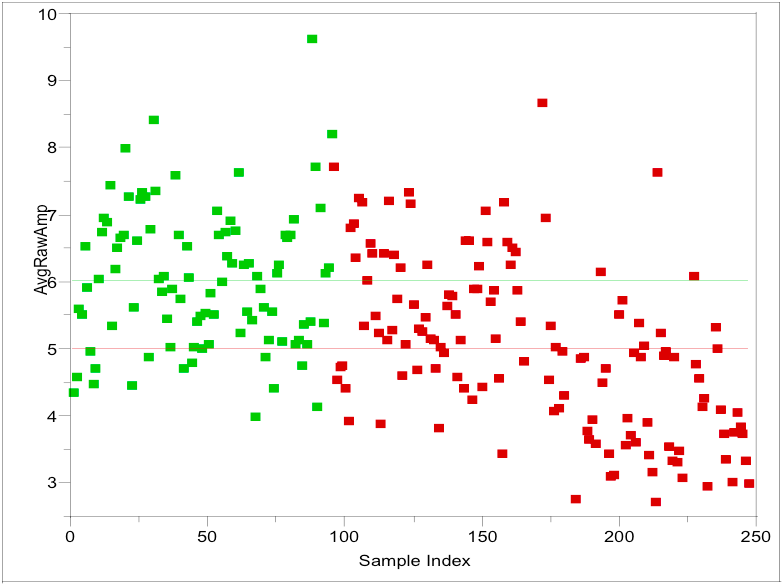
\includegraphics[width=120mm]{cancer.jpg}
\caption{ Overian cancer dataset with bivirate fit of average amplitude with given samples. The plot is referenced from $http://home.ccr.cancer.gov/ncifdaproteomics/ppatterns.asp$ \label{problem1Pic2}}
\end{figure}
\par
From both figures, we can see that the datasets do not form a manifold, meaning it is applicable to PCA. 

\section{Implementation}
Since neither of the datasets come with the testing data, I have to split the set into training and testing samples. For the iris flower dataset, the total number of samples are 150, so I use 20 of them as testing data. For the overian cancer dataset, the total number of samples are 216, and I use 30 of them as my testing set. All the testing samples are randomly extracted from the datasets. Also, training samples and testing samples are mutually exclusive.\par
I recycled my PCA code from assignment 3 to get the principle components of the given datasets.The function implemented in assignment 3, $[components, variances]=pca(XS,m)$, is used to take training set $XS$ and number of components to be extracted, $m$, as inputs. The output, $components$, is what I use to feed to SVM training model. In the SVM-only case, I just feed raw dataset to SVM training models.\par

In terms of SVM, instead of using default matlab toolbox, I use LIBSVM open source library from National Taiwan University. The advantage of this library is that when data follows gaussian distribution, we can adjust the $\sigma$ value in the gaussian kernel:
\[G (X, \sigma) = \frac{1}{(\sqrt{2\pi}\sigma)^N}\exp(\frac{-\|X\| ^2}{2\sigma ^2})\]
Where $N$ is the number of samples, and X is the data to be trained. Fine tuning $\sigma$ in SVM problems is very important as it determines how relaxed the fited curve is. However, in this project, we are trying to get the performance gain/loss with PCA, so the $\sigma$ value is fixed to $1$ in this case. The LIBSVM library allows us to prototype the learning model with only two function calls, $model = svmtrain(label, data, \sigma, kernel)$ and $accuracy = svmtest(testing label, testing data, model)$. Most of the input parameters are quite self-explaintory other than $kernel$ in $svmtrain$. $kernel$ is passed on as a integer flags. In our case, we use $2$ indicating gaussian kernel.\par
I have attached my source code as well as essential toolbox (for LIBSVM) in the package. Feel free to run the program.   

\section{Benchmark}
The benchmarks I have been running focus on two aspects of the results, program execution time and testing accuracy. The parameters such as $\sigma$ and $kernel$ are fixed for both programs (PCA-SVM and SVM-Only).The figures below present all forms of benchmarks results alone with their explainations. Each of the data points are taken as the average of 5 attempts as every PCA function call can produce different principle components and therefore produce different results.

\begin{figure}[H]
\centering
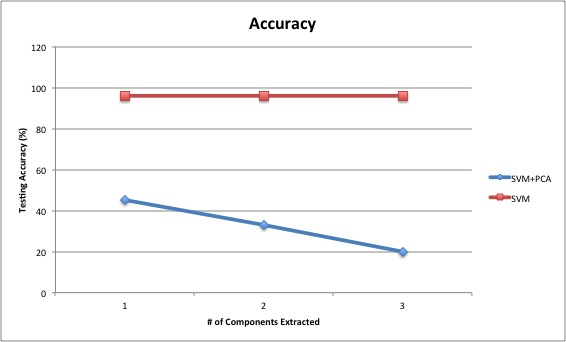
\includegraphics[width=120mm]{iris_accuracy.jpg}
\caption{ This is the accuracy plot for iris flowers dataset, from what I can see, the accuracy reduecd dramaticly. I have anticipated accuracy drop from PCA. One of the possible reason is that the training set only has 120 observations, making the training less effective while the principle components are extracted. Also, since the PCA-only model does not have variables like total number of principle components to be extracted, I use constant SVM-Only results for simplicity.\label{problem1Pic2}}
\end{figure}

\begin{figure}[H]
\centering
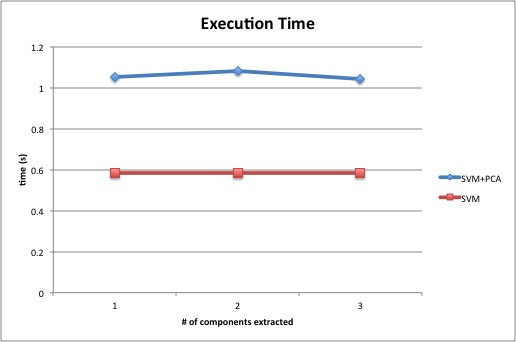
\includegraphics[width=120mm]{iris_time.jpg}
\caption{ This is the execution time plot for iris flower dataset. I see negative speedups while using PCA. The main reason is that the original dataset only has 4 attributes, which makes raw data processing simple enough. \label{problem1Pic2}}
\end{figure}

\begin{figure}[H]
\centering
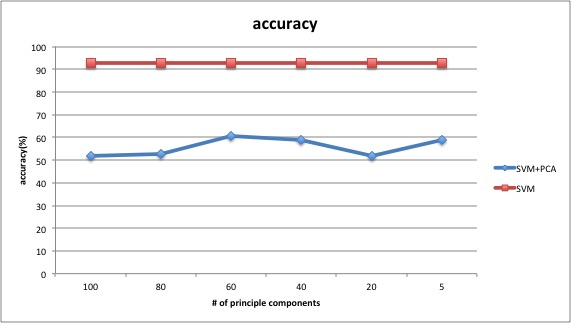
\includegraphics[width=120mm]{cancer_accuracy.jpg}
\caption{ This is the accuracy plot for Overian cancer patients, Though the accuracy still is much less than SVM-Only model, it is far better than the iris flowers case. Part of the reason is that this dataset has almost 200 training set. Nevertheless, the PCA still produces significant erros for the SVM model. Also, another drawback is that the extractable principle components are limited by total number of observations in the training set. We cannot extract, for example, 3000 principle components as we only have 200 training points, and that is also the reason for the errors. \label{problem1Pic2}}
\end{figure}

\begin{figure}[H]
\centering
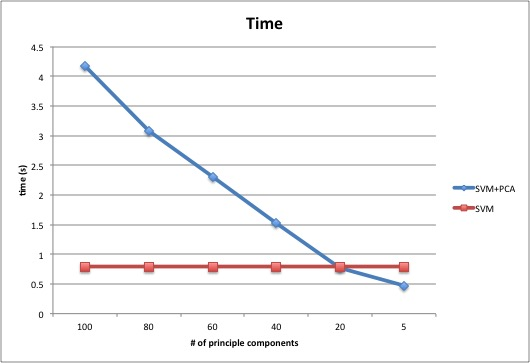
\includegraphics[width=120mm]{cancer_time.jpg}
\caption{ This is the time plot for Overian cancer patients. Unlike previous benchmarks, the time comparsion for the overian cancer shows advantages of PCA. As I reduce the number of principle components, the execution time drops rapidly. When the number of principle components is 3, the program has positve speedups against SVM-only model. \label{problem1Pic2}}
\end{figure}

\section{Conclusion}
I see that no matter how big the datset is, PCA will always reduce the prediction accuracy. Intuitively speaking, it makes sense as PCA basically extracts the eigenvalues of important features and thus reduces the resolutions of the raw datasets. However, when the dataset is huge (in hundreds of megabytes range, given the overian cancer dataset is about 31 megabytes), PCA will have sufficient speedups against raw classification problems. From what I see, PCA is not really necessary when it comes to classification, given we already have efficient and accurate solutions like SVM, neural nets, and logistic regression. PCA simply brings an option to trade-in accuracy with training speedups. When the training time less important than accuracy, PCA is not a better solution to go with. 
\end{document}

